% Options for packages loaded elsewhere
\PassOptionsToPackage{unicode}{hyperref}
\PassOptionsToPackage{hyphens}{url}
%
\documentclass[
]{article}
\usepackage{amsmath,amssymb}
\usepackage{lmodern}
\usepackage{ifxetex,ifluatex}
\ifnum 0\ifxetex 1\fi\ifluatex 1\fi=0 % if pdftex
  \usepackage[T1]{fontenc}
  \usepackage[utf8]{inputenc}
  \usepackage{textcomp} % provide euro and other symbols
\else % if luatex or xetex
  \usepackage{unicode-math}
  \defaultfontfeatures{Scale=MatchLowercase}
  \defaultfontfeatures[\rmfamily]{Ligatures=TeX,Scale=1}
\fi
% Use upquote if available, for straight quotes in verbatim environments
\IfFileExists{upquote.sty}{\usepackage{upquote}}{}
\IfFileExists{microtype.sty}{% use microtype if available
  \usepackage[]{microtype}
  \UseMicrotypeSet[protrusion]{basicmath} % disable protrusion for tt fonts
}{}
\makeatletter
\@ifundefined{KOMAClassName}{% if non-KOMA class
  \IfFileExists{parskip.sty}{%
    \usepackage{parskip}
  }{% else
    \setlength{\parindent}{0pt}
    \setlength{\parskip}{6pt plus 2pt minus 1pt}}
}{% if KOMA class
  \KOMAoptions{parskip=half}}
\makeatother
\usepackage{xcolor}
\IfFileExists{xurl.sty}{\usepackage{xurl}}{} % add URL line breaks if available
\IfFileExists{bookmark.sty}{\usepackage{bookmark}}{\usepackage{hyperref}}
\hypersetup{
  pdftitle={Assignment1},
  hidelinks,
  pdfcreator={LaTeX via pandoc}}
\urlstyle{same} % disable monospaced font for URLs
\usepackage[margin=1in]{geometry}
\usepackage{color}
\usepackage{fancyvrb}
\newcommand{\VerbBar}{|}
\newcommand{\VERB}{\Verb[commandchars=\\\{\}]}
\DefineVerbatimEnvironment{Highlighting}{Verbatim}{commandchars=\\\{\}}
% Add ',fontsize=\small' for more characters per line
\usepackage{framed}
\definecolor{shadecolor}{RGB}{248,248,248}
\newenvironment{Shaded}{\begin{snugshade}}{\end{snugshade}}
\newcommand{\AlertTok}[1]{\textcolor[rgb]{0.94,0.16,0.16}{#1}}
\newcommand{\AnnotationTok}[1]{\textcolor[rgb]{0.56,0.35,0.01}{\textbf{\textit{#1}}}}
\newcommand{\AttributeTok}[1]{\textcolor[rgb]{0.77,0.63,0.00}{#1}}
\newcommand{\BaseNTok}[1]{\textcolor[rgb]{0.00,0.00,0.81}{#1}}
\newcommand{\BuiltInTok}[1]{#1}
\newcommand{\CharTok}[1]{\textcolor[rgb]{0.31,0.60,0.02}{#1}}
\newcommand{\CommentTok}[1]{\textcolor[rgb]{0.56,0.35,0.01}{\textit{#1}}}
\newcommand{\CommentVarTok}[1]{\textcolor[rgb]{0.56,0.35,0.01}{\textbf{\textit{#1}}}}
\newcommand{\ConstantTok}[1]{\textcolor[rgb]{0.00,0.00,0.00}{#1}}
\newcommand{\ControlFlowTok}[1]{\textcolor[rgb]{0.13,0.29,0.53}{\textbf{#1}}}
\newcommand{\DataTypeTok}[1]{\textcolor[rgb]{0.13,0.29,0.53}{#1}}
\newcommand{\DecValTok}[1]{\textcolor[rgb]{0.00,0.00,0.81}{#1}}
\newcommand{\DocumentationTok}[1]{\textcolor[rgb]{0.56,0.35,0.01}{\textbf{\textit{#1}}}}
\newcommand{\ErrorTok}[1]{\textcolor[rgb]{0.64,0.00,0.00}{\textbf{#1}}}
\newcommand{\ExtensionTok}[1]{#1}
\newcommand{\FloatTok}[1]{\textcolor[rgb]{0.00,0.00,0.81}{#1}}
\newcommand{\FunctionTok}[1]{\textcolor[rgb]{0.00,0.00,0.00}{#1}}
\newcommand{\ImportTok}[1]{#1}
\newcommand{\InformationTok}[1]{\textcolor[rgb]{0.56,0.35,0.01}{\textbf{\textit{#1}}}}
\newcommand{\KeywordTok}[1]{\textcolor[rgb]{0.13,0.29,0.53}{\textbf{#1}}}
\newcommand{\NormalTok}[1]{#1}
\newcommand{\OperatorTok}[1]{\textcolor[rgb]{0.81,0.36,0.00}{\textbf{#1}}}
\newcommand{\OtherTok}[1]{\textcolor[rgb]{0.56,0.35,0.01}{#1}}
\newcommand{\PreprocessorTok}[1]{\textcolor[rgb]{0.56,0.35,0.01}{\textit{#1}}}
\newcommand{\RegionMarkerTok}[1]{#1}
\newcommand{\SpecialCharTok}[1]{\textcolor[rgb]{0.00,0.00,0.00}{#1}}
\newcommand{\SpecialStringTok}[1]{\textcolor[rgb]{0.31,0.60,0.02}{#1}}
\newcommand{\StringTok}[1]{\textcolor[rgb]{0.31,0.60,0.02}{#1}}
\newcommand{\VariableTok}[1]{\textcolor[rgb]{0.00,0.00,0.00}{#1}}
\newcommand{\VerbatimStringTok}[1]{\textcolor[rgb]{0.31,0.60,0.02}{#1}}
\newcommand{\WarningTok}[1]{\textcolor[rgb]{0.56,0.35,0.01}{\textbf{\textit{#1}}}}
\usepackage{graphicx}
\makeatletter
\def\maxwidth{\ifdim\Gin@nat@width>\linewidth\linewidth\else\Gin@nat@width\fi}
\def\maxheight{\ifdim\Gin@nat@height>\textheight\textheight\else\Gin@nat@height\fi}
\makeatother
% Scale images if necessary, so that they will not overflow the page
% margins by default, and it is still possible to overwrite the defaults
% using explicit options in \includegraphics[width, height, ...]{}
\setkeys{Gin}{width=\maxwidth,height=\maxheight,keepaspectratio}
% Set default figure placement to htbp
\makeatletter
\def\fps@figure{htbp}
\makeatother
\setlength{\emergencystretch}{3em} % prevent overfull lines
\providecommand{\tightlist}{%
  \setlength{\itemsep}{0pt}\setlength{\parskip}{0pt}}
\setcounter{secnumdepth}{-\maxdimen} % remove section numbering
\ifluatex
  \usepackage{selnolig}  % disable illegal ligatures
\fi

\title{Assignment1}
\author{}
\date{\vspace{-2.5em}}

\begin{document}
\maketitle

\#\#\#Assignment 1 Jop Keuning 11014407, Nienke Deutz 2732866 and
Harshita Choudhary 13807609

\#\#Exercise1

\#1a First of we check the data for normality which is done in two ways,
first with a qqplot which shows that normality is present.

\begin{Shaded}
\begin{Highlighting}[]
\NormalTok{waiting\_times }\OtherTok{\textless{}{-}} \FunctionTok{c}\NormalTok{(}\FloatTok{5.4}\NormalTok{, }\FloatTok{17.9}\NormalTok{, }\FloatTok{19.0}\NormalTok{, }\FloatTok{0.5}\NormalTok{, }\FloatTok{15.9}\NormalTok{, }\FloatTok{2.7}\NormalTok{, }\FloatTok{6.2}\NormalTok{, }\FloatTok{2.5}\NormalTok{, }\FloatTok{4.7}\NormalTok{, }\FloatTok{6.9}\NormalTok{, }\FloatTok{10.8}\NormalTok{, }\FloatTok{24.3}\NormalTok{, }\FloatTok{5.6}\NormalTok{, }\FloatTok{23.0}\NormalTok{, }\FloatTok{10.7}\NormalTok{)}
\NormalTok{mu }\OtherTok{\textless{}{-}} \FunctionTok{mean}\NormalTok{(waiting\_times)}
\NormalTok{sigma }\OtherTok{\textless{}{-}} \FunctionTok{sd}\NormalTok{(waiting\_times)}
\FunctionTok{qqnorm}\NormalTok{(waiting\_times)}
\end{Highlighting}
\end{Shaded}

\includegraphics{assignment1_files/figure-latex/unnamed-chunk-1-1.pdf}

But to be extra sure that normality is indeed the case a shapiro test
will confirm it as indeed fufilling the normality condition

\begin{Shaded}
\begin{Highlighting}[]
\FunctionTok{shapiro.test}\NormalTok{(waiting\_times)}
\end{Highlighting}
\end{Shaded}

\begin{verbatim}
## 
##  Shapiro-Wilk normality test
## 
## data:  waiting_times
## W = 0.90744, p-value = 0.1237
\end{verbatim}

Now that normality has been confirmed it is time to construct a
confidence interval for the mu at 97\% for which alpha needs to be set
at 0.05. With this the confidence interval and the minimum sample size
can be found.

To calculate the confidence interval we take the mean of the data we
take upper quantile of the normal distribution as za with the upper
quantile taken defined as 1-alpha. With this the confidence is
calculated as
\(mean - (za/2)*sd/squareroot(n) as the lower bound and mean + (za/2)*sd/squareroot(n)\)
where n is the sample size set at 10, mean is the average of the data
and sd the standard deviation

\begin{Shaded}
\begin{Highlighting}[]
\NormalTok{n }\OtherTok{\textless{}{-}} \FunctionTok{length}\NormalTok{(waiting\_times)}

\NormalTok{alpha }\OtherTok{\textless{}{-}} \FloatTok{0.015}
\NormalTok{za }\OtherTok{\textless{}{-}} \FunctionTok{qnorm}\NormalTok{(}\DecValTok{1}\SpecialCharTok{{-}}\NormalTok{alpha)}
\NormalTok{ci }\OtherTok{\textless{}{-}} \FunctionTok{c}\NormalTok{(mu }\SpecialCharTok{{-}}\NormalTok{(za}\SpecialCharTok{/}\DecValTok{2}\NormalTok{)}\SpecialCharTok{*}\NormalTok{(sigma}\SpecialCharTok{/}\FunctionTok{sqrt}\NormalTok{(n)), mu }\SpecialCharTok{+}\NormalTok{ (za}\SpecialCharTok{/}\DecValTok{2}\NormalTok{)}\SpecialCharTok{*}\NormalTok{(sigma}\SpecialCharTok{/}\FunctionTok{sqrt}\NormalTok{(n)))}
\FunctionTok{print}\NormalTok{(ci)}
\end{Highlighting}
\end{Shaded}

\begin{verbatim}
## [1]  8.23295 12.58038
\end{verbatim}

To calculate the minimum sample size needed to attain this confidence
interval a \(za\) value of the normal distribution of \(1-alpha/2\) is
needed. With this the calculation of the minimum number of samples is as
follows: \(n_min = (za^2*sd^2)/E\). Here E signifies the error and the
the confidence interval will have a length of at most 2E. As we want the
length to be at most 2 we can set E equal to 1 resulting in the
followint minimum number of samples

\begin{Shaded}
\begin{Highlighting}[]
\NormalTok{za2 }\OtherTok{\textless{}{-}} \FunctionTok{qnorm}\NormalTok{(}\DecValTok{1}\SpecialCharTok{{-}}\NormalTok{alpha}\SpecialCharTok{/}\DecValTok{2}\NormalTok{)}
\NormalTok{n\_minimum }\OtherTok{\textless{}{-}}\NormalTok{ (za2}\SpecialCharTok{\^{}}\DecValTok{2}\SpecialCharTok{*}\NormalTok{sigma}\SpecialCharTok{\^{}}\DecValTok{2}\NormalTok{)}\SpecialCharTok{/}\DecValTok{1}
\FunctionTok{print}\NormalTok{(n\_minimum)}
\end{Highlighting}
\end{Shaded}

\begin{verbatim}
## [1] 356.1753
\end{verbatim}

Finally we want to compare the previously calculated confidence interval
with a bootstrapped one. The code for this bootstrap and it's result can
be seen below.

\begin{Shaded}
\begin{Highlighting}[]
\NormalTok{B }\OtherTok{=} \DecValTok{1000}
\NormalTok{Tstar }\OtherTok{=} \FunctionTok{numeric}\NormalTok{(B)}
\ControlFlowTok{for}\NormalTok{(i }\ControlFlowTok{in} \DecValTok{1}\SpecialCharTok{:}\NormalTok{B)\{}
\NormalTok{  Xstar }\OtherTok{\textless{}{-}} \FunctionTok{sample}\NormalTok{(waiting\_times, }\AttributeTok{replace =} \ConstantTok{TRUE}\NormalTok{)}
\NormalTok{  Tstar[i] }\OtherTok{\textless{}{-}} \FunctionTok{mean}\NormalTok{(Xstar)\}}
\NormalTok{Tstar015 }\OtherTok{\textless{}{-}} \FunctionTok{quantile}\NormalTok{(Tstar, }\FloatTok{0.015}\NormalTok{)}
\NormalTok{Tstar985 }\OtherTok{\textless{}{-}} \FunctionTok{quantile}\NormalTok{(Tstar, }\FloatTok{0.985}\NormalTok{)}
\FunctionTok{sum}\NormalTok{(Tstar }\SpecialCharTok{\textless{}}\NormalTok{Tstar015)}
\end{Highlighting}
\end{Shaded}

\begin{verbatim}
## [1] 15
\end{verbatim}

\begin{Shaded}
\begin{Highlighting}[]
\NormalTok{boodstrap }\OtherTok{\textless{}{-}} \FunctionTok{c}\NormalTok{(}\DecValTok{2}\SpecialCharTok{*}\NormalTok{mu}\SpecialCharTok{{-}}\NormalTok{Tstar985,}\DecValTok{2}\SpecialCharTok{*}\NormalTok{mu}\SpecialCharTok{{-}}\NormalTok{Tstar015)}
\FunctionTok{print}\NormalTok{(boodstrap)}
\end{Highlighting}
\end{Shaded}

\begin{verbatim}
##     98.5%      1.5% 
##  5.985967 14.507067
\end{verbatim}

When compared to the confidence interval calculated above which looks
like this, (8.23295 12.58038) we can see that the bootstrap confidence
interval is wider than that of the calculated one by a difference of
around 2 in both bounds.

\#1b To verify the doctor's claim we perform both a t-test and a sign
test for a mean less than 15. From the t-test we can see that the mean
lies below 13.94 with a confidence interval of 95\%. With the sign test
we get a probability range of 0.69 to 1 with the confidence interval of
95\% meaning we can say that for both tests the doctor's claim that the
waiting time is less than 15 minutes on average is correct.

\begin{Shaded}
\begin{Highlighting}[]
\NormalTok{ttest }\OtherTok{=} \FunctionTok{t.test}\NormalTok{(waiting\_times,}\AttributeTok{mu=}\DecValTok{15}\NormalTok{,}\AttributeTok{alt=}\StringTok{"less"}\NormalTok{)}
\FunctionTok{print}\NormalTok{(ttest)}
\end{Highlighting}
\end{Shaded}

\begin{verbatim}
## 
##  One Sample t-test
## 
## data:  waiting_times
## t = -2.2928, df = 14, p-value = 0.01893
## alternative hypothesis: true mean is less than 15
## 95 percent confidence interval:
##      -Inf 13.93517
## sample estimates:
## mean of x 
##  10.40667
\end{verbatim}

\begin{Shaded}
\begin{Highlighting}[]
\NormalTok{n }\OtherTok{=} \DecValTok{10}
\FunctionTok{binom.test}\NormalTok{(}\FunctionTok{sum}\NormalTok{(waiting\_times}\SpecialCharTok{\textless{}}\DecValTok{15}\NormalTok{), n)}
\end{Highlighting}
\end{Shaded}

\begin{verbatim}
## 
##  Exact binomial test
## 
## data:  sum(waiting_times < 15) and n
## number of successes = 10, number of trials = 10, p-value = 0.001953
## alternative hypothesis: true probability of success is not equal to 0.5
## 95 percent confidence interval:
##  0.6915029 1.0000000
## sample estimates:
## probability of success 
##                      1
\end{verbatim}

1c.

To compute the power of the t-test and sign test is to use p-value of
different samples from the data for a large amount of iterations and
calculate the average of all p-values that satisfy the condition of
\(p_value < 0.05\), meaning all significant p-values. This results in
that the sign tests have a power of 1 but in both the cases for mu at 13
and 14 the ttest has a power below 0.5

\begin{Shaded}
\begin{Highlighting}[]
\NormalTok{B}\OtherTok{=}\DecValTok{1000}
\NormalTok{n}\OtherTok{\textless{}{-}}\FunctionTok{length}\NormalTok{(waiting\_times)}
\NormalTok{psign}\OtherTok{\textless{}{-}}\FunctionTok{numeric}\NormalTok{(B)}
\NormalTok{pttest}\OtherTok{\textless{}{-}}\FunctionTok{numeric}\NormalTok{(B)}
\ControlFlowTok{for}\NormalTok{(i }\ControlFlowTok{in} \DecValTok{1}\SpecialCharTok{:}\NormalTok{B) \{}
\NormalTok{  x }\OtherTok{=} \FunctionTok{sample}\NormalTok{(waiting\_times, }\AttributeTok{replace =} \ConstantTok{TRUE}\NormalTok{)}
\NormalTok{  pttest[i]}\OtherTok{\textless{}{-}}\FunctionTok{t.test}\NormalTok{(x, }\AttributeTok{mu=}\DecValTok{13}\NormalTok{)[[}\DecValTok{3}\NormalTok{]] }\DocumentationTok{\#\# extract p{-}value}
\NormalTok{  psign[i]}\OtherTok{\textless{}{-}}\FunctionTok{binom.test}\NormalTok{(}\FunctionTok{sum}\NormalTok{(}\AttributeTok{x=}\DecValTok{13}\NormalTok{), n, }\AttributeTok{p=}\FloatTok{0.5}\NormalTok{)[[}\DecValTok{3}\NormalTok{]]}
\NormalTok{\}}
\FunctionTok{sum}\NormalTok{(psign}\SpecialCharTok{\textless{}}\FloatTok{0.05}\NormalTok{)}\SpecialCharTok{/}\NormalTok{B}
\end{Highlighting}
\end{Shaded}

\begin{verbatim}
## [1] 1
\end{verbatim}

\begin{Shaded}
\begin{Highlighting}[]
\FunctionTok{sum}\NormalTok{(pttest}\SpecialCharTok{\textless{}}\FloatTok{0.05}\NormalTok{)}\SpecialCharTok{/}\NormalTok{B}
\end{Highlighting}
\end{Shaded}

\begin{verbatim}
## [1] 0.253
\end{verbatim}

\begin{Shaded}
\begin{Highlighting}[]
\ControlFlowTok{for}\NormalTok{(i }\ControlFlowTok{in} \DecValTok{1}\SpecialCharTok{:}\NormalTok{B) \{}
\NormalTok{  x }\OtherTok{=} \FunctionTok{sample}\NormalTok{(waiting\_times, }\AttributeTok{replace =} \ConstantTok{TRUE}\NormalTok{)}
\NormalTok{  pttest[i]}\OtherTok{\textless{}{-}}\FunctionTok{t.test}\NormalTok{(x, }\AttributeTok{mu=}\DecValTok{14}\NormalTok{)[[}\DecValTok{3}\NormalTok{]] }\DocumentationTok{\#\# extract p{-}value}
\NormalTok{  psign[i]}\OtherTok{\textless{}{-}}\FunctionTok{binom.test}\NormalTok{(}\FunctionTok{sum}\NormalTok{(}\AttributeTok{x=}\DecValTok{14}\NormalTok{), n, }\AttributeTok{p=}\FloatTok{0.5}\NormalTok{)[[}\DecValTok{3}\NormalTok{]]}
\NormalTok{\}}
\FunctionTok{sum}\NormalTok{(psign}\SpecialCharTok{\textless{}}\FloatTok{0.05}\NormalTok{)}\SpecialCharTok{/}\NormalTok{B}
\end{Highlighting}
\end{Shaded}

\begin{verbatim}
## [1] 1
\end{verbatim}

\begin{Shaded}
\begin{Highlighting}[]
\FunctionTok{sum}\NormalTok{(pttest}\SpecialCharTok{\textless{}}\FloatTok{0.05}\NormalTok{)}\SpecialCharTok{/}\NormalTok{B}
\end{Highlighting}
\end{Shaded}

\begin{verbatim}
## [1] 0.404
\end{verbatim}

\#\#Exercise 2

\#b

\begin{Shaded}
\begin{Highlighting}[]
\NormalTok{clouds }\OtherTok{\textless{}{-}} \FunctionTok{read.csv}\NormalTok{(}\StringTok{"clouds.txt"}\NormalTok{, }\AttributeTok{sep=}\StringTok{""}\NormalTok{)}
\FunctionTok{is.data.frame}\NormalTok{(clouds)}
\end{Highlighting}
\end{Shaded}

\begin{verbatim}
## [1] TRUE
\end{verbatim}

\begin{Shaded}
\begin{Highlighting}[]
\NormalTok{clouds\_copy }\OtherTok{\textless{}{-}} \FunctionTok{data.frame}\NormalTok{(clouds)}
\NormalTok{clouds\_copy}\SpecialCharTok{$}\NormalTok{square\_root\_seeded }\OtherTok{=}\StringTok{\textquotesingle{}\^{}\textquotesingle{}}\NormalTok{(clouds\_copy}\SpecialCharTok{$}\NormalTok{seeded,}\DecValTok{1}\SpecialCharTok{/}\DecValTok{2}\NormalTok{)}
\NormalTok{clouds\_copy}\SpecialCharTok{$}\NormalTok{square\_root\_unseeded }\OtherTok{=}\StringTok{\textquotesingle{}\^{}\textquotesingle{}}\NormalTok{(clouds\_copy}\SpecialCharTok{$}\NormalTok{unseeded,}\DecValTok{1}\SpecialCharTok{/}\DecValTok{2}\NormalTok{)}
\NormalTok{clouds\_copy}\SpecialCharTok{$}\NormalTok{double\_square\_root\_seeded}\OtherTok{=}\StringTok{\textquotesingle{}\^{}\textquotesingle{}}\NormalTok{(clouds\_copy}\SpecialCharTok{$}\NormalTok{square\_root\_seeded,}\DecValTok{1}\SpecialCharTok{/}\DecValTok{2}\NormalTok{)}
\NormalTok{clouds\_copy}\SpecialCharTok{$}\NormalTok{double\_square\_root\_unseeded}\OtherTok{=}\StringTok{\textquotesingle{}\^{}\textquotesingle{}}\NormalTok{(clouds\_copy}\SpecialCharTok{$}\NormalTok{square\_root\_unseeded,}\DecValTok{1}\SpecialCharTok{/}\DecValTok{2}\NormalTok{)}
\CommentTok{\#View(clouds\_copy)}
\end{Highlighting}
\end{Shaded}

Square root of the values:

\includegraphics{assignment1_files/figure-latex/Normality Check-1.pdf}
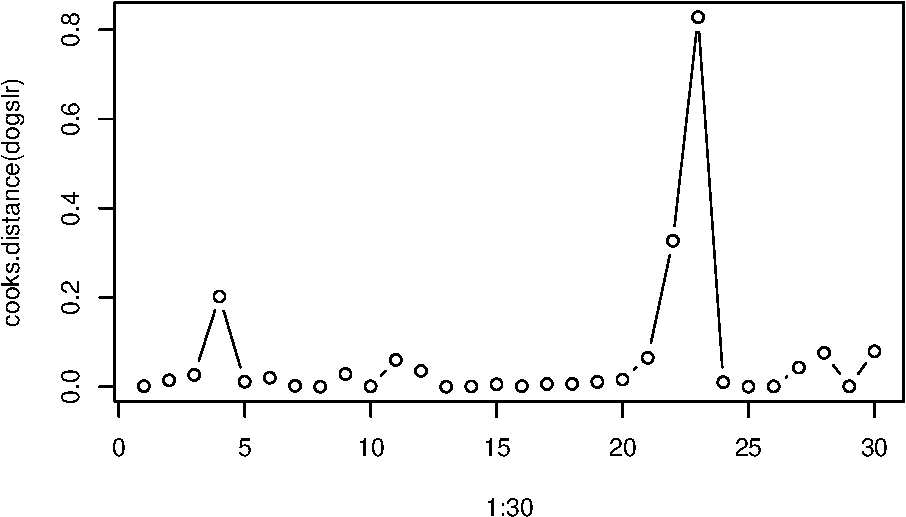
\includegraphics{assignment1_files/figure-latex/unnamed-chunk-9-1.pdf}

QQ - data deviates at the tail. It doesn't seem to follow a normal
distribution. There are a few outliers.

Two Sample T-test:

\begin{verbatim}
## 
##  Paired t-test
## 
## data:  clouds_copy[["square_root_seeded"]] and clouds_copy[["square_root_unseeded"]]
## t = 2.682, df = 25, p-value = 0.01278
## alternative hypothesis: true difference in means is not equal to 0
## 95 percent confidence interval:
##   1.656326 12.617061
## sample estimates:
## mean of the differences 
##                7.136693
\end{verbatim}

p-value is 0.0127 therefore, H0 is rejected. Hence, nitrate has an
effect.

Mann-Whitney Test:

\begin{verbatim}
## Warning in wilcox.test.default(clouds_copy[["square_root_seeded"]],
## clouds_copy[["square_root_unseeded"]]): cannot compute exact p-value with ties
\end{verbatim}

\begin{verbatim}
## 
##  Wilcoxon rank sum test with continuity correction
## 
## data:  clouds_copy[["square_root_seeded"]] and clouds_copy[["square_root_unseeded"]]
## W = 473, p-value = 0.01383
## alternative hypothesis: true location shift is not equal to 0
\end{verbatim}

p-value is 0.0138 less than 0.05 therefore, H0 is rejected. Hence,
nitrate has an effect.

Kolmogorov-Smirnov Test:

\begin{verbatim}
## Warning in ks.test(clouds_copy[["square_root_seeded"]],
## clouds_copy[["square_root_unseeded"]]): cannot compute exact p-value with ties
\end{verbatim}

\begin{verbatim}
## 
##  Two-sample Kolmogorov-Smirnov test
## 
## data:  clouds_copy[["square_root_seeded"]] and clouds_copy[["square_root_unseeded"]]
## D = 0.42308, p-value = 0.01905
## alternative hypothesis: two-sided
\end{verbatim}

p-value is 0.01905 less than 0.05 therefore, H0 is rejected. Hence,
nitrate has an effect.

Double square root values:

\includegraphics{assignment1_files/figure-latex/Normality Check Double Root -1.pdf}
\includegraphics{assignment1_files/figure-latex/unnamed-chunk-10-1.pdf}
QQ : Data deviates at the tails so distribution doesn't seem to be
normal.

Two Sample T-Test:

\begin{verbatim}
## 
##  Paired t-test
## 
## data:  clouds_copy[["double_square_root_seeded"]] and clouds_copy[["double_square_root_unseeded"]]
## t = 2.8413, df = 25, p-value = 0.008811
## alternative hypothesis: true difference in means is not equal to 0
## 95 percent confidence interval:
##  0.2673422 1.6759523
## sample estimates:
## mean of the differences 
##               0.9716472
\end{verbatim}

p-value is 0.008811 therefore, H0 : no effect of silver nitrate, can be
rejected. Hence, nitrate has an effect.

Mann-Whitnney Test:

\begin{verbatim}
## Warning in wilcox.test.default(clouds_copy[["double_square_root_seeded"]], :
## cannot compute exact p-value with ties
\end{verbatim}

\begin{verbatim}
## 
##  Wilcoxon rank sum test with continuity correction
## 
## data:  clouds_copy[["double_square_root_seeded"]] and clouds_copy[["double_square_root_unseeded"]]
## W = 473, p-value = 0.01383
## alternative hypothesis: true location shift is not equal to 0
\end{verbatim}

p-value is 0.01383. Hence, silver nitrate has an effect.

Kolmogorov - Smirnov Test:

\begin{verbatim}
## Warning in ks.test(clouds_copy[["double_square_root_seeded"]],
## clouds_copy[["double_square_root_unseeded"]]): cannot compute exact p-value with
## ties
\end{verbatim}

\begin{verbatim}
## 
##  Two-sample Kolmogorov-Smirnov test
## 
## data:  clouds_copy[["double_square_root_seeded"]] and clouds_copy[["double_square_root_unseeded"]]
## D = 0.42308, p-value = 0.01905
## alternative hypothesis: two-sided
\end{verbatim}

p-value is 0.01905. Hence, silver nitrate has an effect.

Conclusion: The p-value of two sample T-test is lower when the square
root of the data is taken. However, for Mann Whitney and Kolmogorov -
Smirnov Test, the p-value doesn't change on taking the square root.

\#2c

\begin{Shaded}
\begin{Highlighting}[]
\CommentTok{\#Calculate the  mean}
\NormalTok{mean\_estimator }\OtherTok{=} \FunctionTok{mean}\NormalTok{(clouds}\SpecialCharTok{$}\NormalTok{seeded)}
\NormalTok{std\_dev\_estimator }\OtherTok{=} \FunctionTok{sd}\NormalTok{(clouds}\SpecialCharTok{$}\NormalTok{seeded)}
\NormalTok{n }\OtherTok{=} \DecValTok{26}
\FunctionTok{sqrt}\NormalTok{(n)}
\end{Highlighting}
\end{Shaded}

\begin{verbatim}
## [1] 5.09902
\end{verbatim}

\begin{Shaded}
\begin{Highlighting}[]
\NormalTok{t\_0}\FloatTok{.025} \OtherTok{=} \FloatTok{2.05954} 
\NormalTok{c\_i\_lower }\OtherTok{=}\NormalTok{ mean\_estimator }\SpecialCharTok{{-}}\NormalTok{ t\_0}\FloatTok{.025}\SpecialCharTok{*}\NormalTok{std\_dev\_estimator}\SpecialCharTok{/}\FunctionTok{sqrt}\NormalTok{(n)}
\NormalTok{c\_i\_upper }\OtherTok{=}\NormalTok{ mean\_estimator }\SpecialCharTok{+}\NormalTok{ t\_0}\FloatTok{.025}\SpecialCharTok{*}\NormalTok{std\_dev\_estimator}\SpecialCharTok{/}\FunctionTok{sqrt}\NormalTok{(n)}
\NormalTok{c\_i\_lower}
\end{Highlighting}
\end{Shaded}

\begin{verbatim}
## [1] 179.1258
\end{verbatim}

\begin{Shaded}
\begin{Highlighting}[]
\NormalTok{c\_i\_upper}
\end{Highlighting}
\end{Shaded}

\begin{verbatim}
## [1] 704.8434
\end{verbatim}

\begin{Shaded}
\begin{Highlighting}[]
\FunctionTok{t.test}\NormalTok{(clouds[[}\StringTok{\textquotesingle{}seeded\textquotesingle{}}\NormalTok{]],}\AttributeTok{mu =} \DecValTok{0}\NormalTok{)}
\end{Highlighting}
\end{Shaded}

\begin{verbatim}
## 
##  One Sample t-test
## 
## data:  clouds[["seeded"]]
## t = 3.463, df = 25, p-value = 0.001937
## alternative hypothesis: true mean is not equal to 0
## 95 percent confidence interval:
##  179.1260 704.8432
## sample estimates:
## mean of x 
##  441.9846
\end{verbatim}

\begin{Shaded}
\begin{Highlighting}[]
\NormalTok{estimator\_lambda }\OtherTok{=} \DecValTok{1}\SpecialCharTok{/}\NormalTok{mean\_estimator}
\NormalTok{ci\_lower }\OtherTok{=} \DecValTok{1}\SpecialCharTok{/}\FloatTok{704.8432}
\NormalTok{ci\_upper }\OtherTok{=} \DecValTok{1}\SpecialCharTok{/}\FloatTok{179.1260}
\NormalTok{estimator\_lambda}
\end{Highlighting}
\end{Shaded}

\begin{verbatim}
## [1] 0.002262522
\end{verbatim}

\begin{Shaded}
\begin{Highlighting}[]
\NormalTok{ci\_lower}
\end{Highlighting}
\end{Shaded}

\begin{verbatim}
## [1] 0.001418755
\end{verbatim}

\begin{Shaded}
\begin{Highlighting}[]
\NormalTok{ci\_upper}
\end{Highlighting}
\end{Shaded}

\begin{verbatim}
## [1] 0.005582662
\end{verbatim}

lambda(Estimator) = 0.002262522 and confidence interval is
(0.001418755,0.005582662)

Bootstrap Test:

\begin{Shaded}
\begin{Highlighting}[]
\NormalTok{T }\OtherTok{=} \FunctionTok{median}\NormalTok{(clouds[[}\StringTok{\textquotesingle{}seeded\textquotesingle{}}\NormalTok{]])}
\NormalTok{T}
\end{Highlighting}
\end{Shaded}

\begin{verbatim}
## [1] 221.6
\end{verbatim}

\begin{Shaded}
\begin{Highlighting}[]
\NormalTok{B}\OtherTok{=}\DecValTok{1000}
\NormalTok{tstar}\OtherTok{=}\FunctionTok{numeric}\NormalTok{(B)}
\NormalTok{n}\OtherTok{=}\DecValTok{26}

\ControlFlowTok{for}\NormalTok{ (i }\ControlFlowTok{in} \DecValTok{1}\SpecialCharTok{:}\NormalTok{B)\{}
\NormalTok{  xstar}\OtherTok{=}\FunctionTok{rexp}\NormalTok{(n,estimator\_lambda)}
\NormalTok{  tstar[i]}\OtherTok{=}\FunctionTok{median}\NormalTok{(xstar)\}}
\FunctionTok{hist}\NormalTok{(tstar)}
\end{Highlighting}
\end{Shaded}

\includegraphics{assignment1_files/figure-latex/unnamed-chunk-13-1.pdf}

\begin{Shaded}
\begin{Highlighting}[]
\NormalTok{pl}\OtherTok{=}\FunctionTok{sum}\NormalTok{(tstar}\SpecialCharTok{\textless{}}\NormalTok{T)}\SpecialCharTok{/}\NormalTok{B; pr}\OtherTok{=}\FunctionTok{sum}\NormalTok{(tstar}\SpecialCharTok{\textgreater{}}\NormalTok{T)}\SpecialCharTok{/}\NormalTok{B; p}\OtherTok{=}\DecValTok{2}\SpecialCharTok{*}\FunctionTok{min}\NormalTok{(pl,pr)}
\NormalTok{pl;pr;p}
\end{Highlighting}
\end{Shaded}

\begin{verbatim}
## [1] 0.108
\end{verbatim}

\begin{verbatim}
## [1] 0.892
\end{verbatim}

\begin{verbatim}
## [1] 0.216
\end{verbatim}

We get p = 0.266 which is greater than 0.05 therefore, we can't reject
the null hypothesis : seeded data belongs to exponential distribution of
a rate parameter lambda.

kolmogorov - Smirnov Test:

\begin{Shaded}
\begin{Highlighting}[]
\DocumentationTok{\#\# kolmogorov {-} smirnov Test}
\FunctionTok{ks.test}\NormalTok{(}\AttributeTok{x =}\NormalTok{ clouds[[}\StringTok{\textquotesingle{}seeded\textquotesingle{}}\NormalTok{]], }\AttributeTok{y =} \StringTok{"pexp"}\NormalTok{, }\AttributeTok{rate =}\NormalTok{ estimator\_lambda)}
\end{Highlighting}
\end{Shaded}

\begin{verbatim}
## Warning in ks.test(x = clouds[["seeded"]], y = "pexp", rate = estimator_lambda):
## ties should not be present for the Kolmogorov-Smirnov test
\end{verbatim}

\begin{verbatim}
## 
##  One-sample Kolmogorov-Smirnov test
## 
## data:  clouds[["seeded"]]
## D = 0.20035, p-value = 0.2476
## alternative hypothesis: two-sided
\end{verbatim}

We get p = 0.2476 which is greater than 0.05 therefore, we can't reject
the null hypothesis : that seeded data belongs to exponential
distribution of a rate parameter lambda.

\#2d :

\begin{verbatim}
## [1] 17
\end{verbatim}

\begin{verbatim}
## 
##  Exact binomial test
## 
## data:  x and n
## number of successes = 17, number of trials = 26, p-value = 0.9622
## alternative hypothesis: true probability of success is less than 0.5
## 95 percent confidence interval:
##  0.0000000 0.8060396
## sample estimates:
## probability of success 
##              0.6538462
\end{verbatim}

We get a p-value of 0.9622, therefore we can't reject the null
hypothesis that the median is greater than or equal to 300. We can say
with 95\% sugnificance level that the median is not less than 300.

\begin{verbatim}
## 
##  Exact binomial test
## 
## data:  num_less_30 and n
## number of successes = 3, number of trials = 26, p-value = 0.08019
## alternative hypothesis: true probability of success is less than 0.25
## 95 percent confidence interval:
##  0.000000 0.271902
## sample estimates:
## probability of success 
##              0.1153846
\end{verbatim}

p-value is 0.08019. Therefore, we reject that at most 25\% of seeded
clouds have precipitation less than 30 with significance level of 95\%.

\#\#exercise 3

\begin{verbatim}
## [1] TRUE
\end{verbatim}

\#3a
\includegraphics{assignment1_files/figure-latex/unnamed-chunk-16-1.pdf}
QQ plot deivaties at the tail. It doesn't seem to follow a normal
distribution.

\begin{Shaded}
\begin{Highlighting}[]
\FunctionTok{shapiro.test}\NormalTok{(dogs[,}\DecValTok{1}\NormalTok{])}
\end{Highlighting}
\end{Shaded}

\begin{verbatim}
## 
##  Shapiro-Wilk normality test
## 
## data:  dogs[, 1]
## W = 0.83093, p-value = 0.03434
\end{verbatim}

p-value of shapiro-test is less than 0.05 therefore the claim that it
follows a normal distribution is rejected.

\begin{Shaded}
\begin{Highlighting}[]
\FunctionTok{qqnorm}\NormalTok{(dogs[,}\DecValTok{2}\NormalTok{], }\AttributeTok{main=}\StringTok{"QQ plot for halothane"}\NormalTok{); }\FunctionTok{qqline}\NormalTok{(dogs[,}\DecValTok{2}\NormalTok{])}
\end{Highlighting}
\end{Shaded}

\includegraphics{assignment1_files/figure-latex/unnamed-chunk-18-1.pdf}
Looking at the QQ-plot it is reasonable to say that Halothane data is
from a normal distribution.

\begin{Shaded}
\begin{Highlighting}[]
\FunctionTok{shapiro.test}\NormalTok{(dogs[,}\DecValTok{2}\NormalTok{])}
\end{Highlighting}
\end{Shaded}

\begin{verbatim}
## 
##  Shapiro-Wilk normality test
## 
## data:  dogs[, 2]
## W = 0.9234, p-value = 0.3862
\end{verbatim}

shapiro test p-value is greater than 0.05. It follows a normal
distribution.

\begin{Shaded}
\begin{Highlighting}[]
\FunctionTok{qqnorm}\NormalTok{(dogs[,}\DecValTok{3}\NormalTok{],}\AttributeTok{main =} \StringTok{"QQ plot for cyclopropane"}\NormalTok{); }\FunctionTok{qqline}\NormalTok{(dogs[,}\DecValTok{3}\NormalTok{])}
\end{Highlighting}
\end{Shaded}

\includegraphics{assignment1_files/figure-latex/unnamed-chunk-20-1.pdf}
Very less diviation therefore, we can say that it comes from a normal
distribution.

\begin{Shaded}
\begin{Highlighting}[]
\FunctionTok{shapiro.test}\NormalTok{(dogs[,}\DecValTok{3}\NormalTok{])}
\end{Highlighting}
\end{Shaded}

\begin{verbatim}
## 
##  Shapiro-Wilk normality test
## 
## data:  dogs[, 3]
## W = 0.93334, p-value = 0.4815
\end{verbatim}

shapiro test p-value is greater than 0.05. It follows a normal
distribution.

\#3b

CORRELATION TEST :

\begin{verbatim}
## Warning in cor.test.default(dogs[["isofluorane"]], dogs[["halothane"]], : Cannot
## compute exact p-value with ties
\end{verbatim}

\begin{verbatim}
## 
##  Spearman's rank correlation rho
## 
## data:  dogs[["isofluorane"]] and dogs[["halothane"]]
## S = 128.89, p-value = 0.5436
## alternative hypothesis: true rho is not equal to 0
## sample estimates:
##      rho 
## 0.218846
\end{verbatim}

p value of 0.5 is greater than 0.05 therefore, we can't reject the null
hypothesis that there is no linear correlation. Hence, isofluorane and
halothane are not linearly correlated.

\includegraphics{assignment1_files/figure-latex/unnamed-chunk-22-1.pdf}
QQ plot - Very less diviation therefore, we can say that it comes from a
normal distribution.

\begin{verbatim}
## 
##  Shapiro-Wilk normality test
## 
## data:  dogs[, 1] - dogs[, 2]
## W = 0.96828, p-value = 0.8744
\end{verbatim}

shapiro test p-value is 0.8744 which is greater than 0.05. Therefore,
the difference in isofluorane and halothane is normally distributed.

Two paired sample T-Test :

\begin{verbatim}
## 
##  Paired t-test
## 
## data:  dogs[, 1] and dogs[, 2]
## t = -0.37755, df = 9, p-value = 0.7145
## alternative hypothesis: true difference in means is not equal to 0
## 95 percent confidence interval:
##  -0.2447093  0.1747093
## sample estimates:
## mean of the differences 
##                  -0.035
\end{verbatim}

p value of 0.7145 is more than 0.05, therefore there is no difference
between the effect of isofluorane and halothane. Distribution of these
columns are not significantly different.

PERMUTATION TEST:

\begin{Shaded}
\begin{Highlighting}[]
\FunctionTok{boxplot}\NormalTok{(dogs[,}\DecValTok{1}\NormalTok{],dogs[,}\DecValTok{2}\NormalTok{],}\AttributeTok{names=}\FunctionTok{c}\NormalTok{(}\StringTok{"isoflurane"}\NormalTok{,}\StringTok{"halothane"}\NormalTok{))}
\end{Highlighting}
\end{Shaded}

\includegraphics{assignment1_files/figure-latex/permuttaion test-1.pdf}

\begin{Shaded}
\begin{Highlighting}[]
\NormalTok{mystat}\OtherTok{=}\ControlFlowTok{function}\NormalTok{(x,y) \{}\FunctionTok{mean}\NormalTok{(x}\SpecialCharTok{{-}}\NormalTok{y)\}}
\NormalTok{B}\OtherTok{=}\DecValTok{1000}\NormalTok{; tstar}\OtherTok{=}\FunctionTok{numeric}\NormalTok{(B)}
\ControlFlowTok{for}\NormalTok{ (i }\ControlFlowTok{in} \DecValTok{1}\SpecialCharTok{:}\NormalTok{B) \{}
\NormalTok{  dogstar}\OtherTok{=}\FunctionTok{t}\NormalTok{(}\FunctionTok{apply}\NormalTok{(}\FunctionTok{cbind}\NormalTok{(dogs[,}\DecValTok{1}\NormalTok{],dogs[,}\DecValTok{2}\NormalTok{]),}\DecValTok{1}\NormalTok{,sample))}
\NormalTok{  tstar[i]}\OtherTok{=}\FunctionTok{mystat}\NormalTok{(dogstar[,}\DecValTok{1}\NormalTok{],dogstar[,}\DecValTok{2}\NormalTok{]) \}}

\NormalTok{myt}\OtherTok{=}\FunctionTok{mystat}\NormalTok{(dogs[,}\DecValTok{1}\NormalTok{],dogs[,}\DecValTok{2}\NormalTok{])}
\CommentTok{\#myt}
\FunctionTok{hist}\NormalTok{(tstar)}
\end{Highlighting}
\end{Shaded}

\includegraphics{assignment1_files/figure-latex/unnamed-chunk-25-1.pdf}

\begin{Shaded}
\begin{Highlighting}[]
\NormalTok{pl}\OtherTok{=}\FunctionTok{sum}\NormalTok{(tstar}\SpecialCharTok{\textless{}}\NormalTok{myt)}\SpecialCharTok{/}\NormalTok{B}
\NormalTok{pr}\OtherTok{=}\FunctionTok{sum}\NormalTok{(tstar}\SpecialCharTok{\textgreater{}}\NormalTok{myt)}\SpecialCharTok{/}\NormalTok{B}
\NormalTok{p}\OtherTok{=}\DecValTok{2}\SpecialCharTok{*}\FunctionTok{min}\NormalTok{(pl,pr)}
\NormalTok{p}
\end{Highlighting}
\end{Shaded}

\begin{verbatim}
## [1] 0.664
\end{verbatim}

p value of 0.63 is more than 0.05, therefore there is no difference
between the effect of isofluorane and halothane. Distribution of these
columns are not significantly different

Permutation test for two-paired samples is valid here and it doesn't
depend on the distribution of data. Here, T-test will perform better
than the permutation test because data of difference in isofluorane and
halothane is normally distributed.

\#3c One - way ANOVA:

\begin{verbatim}
## [1] TRUE
\end{verbatim}

\begin{verbatim}
## [1] FALSE
\end{verbatim}

\begin{verbatim}
## Analysis of Variance Table
## 
## Response: yield
##           Df Sum Sq Mean Sq F value Pr(>F)  
## variety    2 1.0808 0.54040   5.355  0.011 *
## Residuals 27 2.7247 0.10092                 
## ---
## Signif. codes:  0 '***' 0.001 '**' 0.01 '*' 0.05 '.' 0.1 ' ' 1
\end{verbatim}

The p-value 0.011, hence HA : μ1 = μ2 = μ3 is is rejected with 95\%
significance level. Therefore, the type of drug has an effect on the
concentration of plasma epinephrine.

\begin{Shaded}
\begin{Highlighting}[]
\FunctionTok{qqnorm}\NormalTok{(}\FunctionTok{residuals}\NormalTok{(dogsanova),}\AttributeTok{main =} \StringTok{"QQ plot of estimated erros"}\NormalTok{) }
\end{Highlighting}
\end{Shaded}

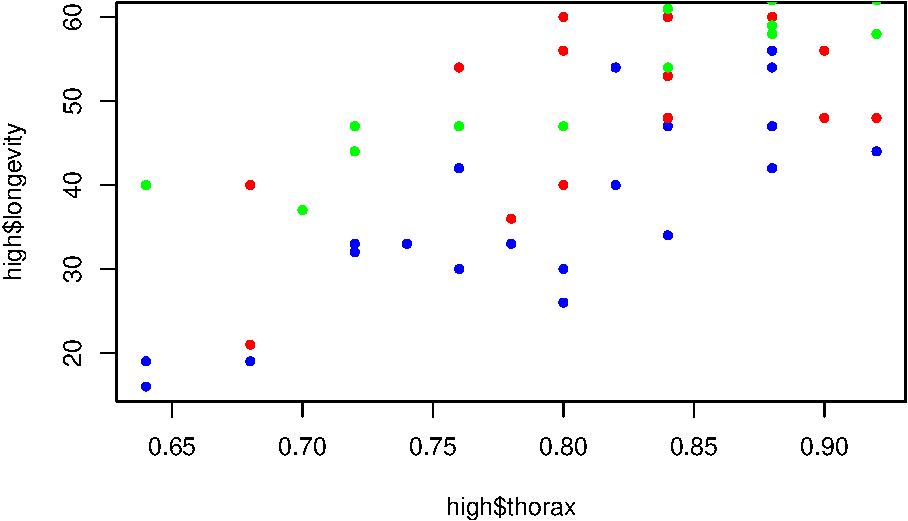
\includegraphics{assignment1_files/figure-latex/unnamed-chunk-28-1.pdf}
QQ plot of residuals eik = Yik − μi (k = 1 to 10 and i = 1 to 3 ) looks
close to a normal distribution.

\begin{Shaded}
\begin{Highlighting}[]
\FunctionTok{plot}\NormalTok{(}\FunctionTok{fitted}\NormalTok{(dogsanova),}\FunctionTok{residuals}\NormalTok{(dogsanova))}
\end{Highlighting}
\end{Shaded}

\includegraphics{assignment1_files/figure-latex/unnamed-chunk-29-1.pdf}
The plot of fitted(group means) against residuals show no pattern.

Therefore, assumptions for one-way ANOVA hold true.

Estimated concentrations of epinephrine for different drugs:

\begin{verbatim}
## [1] 0.434
\end{verbatim}

\begin{verbatim}
## [1] 0.469
\end{verbatim}

\begin{verbatim}
## [1] 0.853
\end{verbatim}

Estimated average concentrations of epinephrine for isoflurane,
halothane and cyclopropane are 0.434,0.469 and 0.853 respectively.

\#3d Krushal-Wallis Test:

\begin{verbatim}
## 
##  Kruskal-Wallis rank sum test
## 
## data:  yield by variety
## Kruskal-Wallis chi-squared = 5.6442, df = 2, p-value = 0.05948
\end{verbatim}

p-value for krushal-wallis test comes out to be 0.05948. Therefore, HA:
μ1 = μ2 = μ3 can't be rejected. The type of drug has no effect on the
concentration of plasma epinephrine.

Conclusion - The reliability of ANOVA test depends on the assumption
that the data comes from a normal dsitribution. Whereas, Krushal-Wallis
Test is a non-paramteric test and doesn't depedent on the distribution
of data. For the above data ANOVA test and Krushal-Wallis Test arrive at
different conclusions. ANOVA test accepts that the type of drug has an
effect on the concentration of plasma epinephrine whereas Krushal-Wallis
test rejects this claim. The above data follows a normal distribution
therefore, the result of one-way ANOVA is more reliable than
Krushal-Wallis Test.

\#\#exercise 5

\#5a

\begin{Shaded}
\begin{Highlighting}[]
\NormalTok{cream }\OtherTok{\textless{}{-}} \FunctionTok{read.csv}\NormalTok{(}\StringTok{"cream.txt"}\NormalTok{, }\AttributeTok{sep=}\StringTok{""}\NormalTok{)}
\FunctionTok{is.vector}\NormalTok{(cream}\SpecialCharTok{$}\NormalTok{acidity)}
\end{Highlighting}
\end{Shaded}

\begin{verbatim}
## [1] TRUE
\end{verbatim}

\begin{Shaded}
\begin{Highlighting}[]
\NormalTok{cream}\SpecialCharTok{$}\NormalTok{batch }\OtherTok{=} \FunctionTok{as.factor}\NormalTok{(cream}\SpecialCharTok{$}\NormalTok{batch)}
\NormalTok{cream}\SpecialCharTok{$}\NormalTok{position }\OtherTok{=} \FunctionTok{as.factor}\NormalTok{(cream}\SpecialCharTok{$}\NormalTok{position)}
\NormalTok{cream}\SpecialCharTok{$}\NormalTok{starter }\OtherTok{=} \FunctionTok{as.factor}\NormalTok{(cream}\SpecialCharTok{$}\NormalTok{starter)}

\NormalTok{creamanov }\OtherTok{=} \FunctionTok{lm}\NormalTok{(acidity}\SpecialCharTok{\textasciitilde{}}\NormalTok{batch}\SpecialCharTok{+}\NormalTok{position}\SpecialCharTok{+}\NormalTok{starter,}\AttributeTok{data=}\NormalTok{cream)}
\FunctionTok{anova}\NormalTok{(creamanov)}
\end{Highlighting}
\end{Shaded}

\begin{verbatim}
## Analysis of Variance Table
## 
## Response: acidity
##           Df Sum Sq Mean Sq F value    Pr(>F)    
## batch      4 18.778  4.6944  8.5975  0.001632 ** 
## position   4  2.348  0.5870  1.0750  0.411191    
## starter    4 44.136 11.0340 20.2080 2.904e-05 ***
## Residuals 12  6.552  0.5460                      
## ---
## Signif. codes:  0 '***' 0.001 '**' 0.01 '*' 0.05 '.' 0.1 ' ' 1
\end{verbatim}

\begin{Shaded}
\begin{Highlighting}[]
\FunctionTok{summary}\NormalTok{(creamanov)}
\end{Highlighting}
\end{Shaded}

\begin{verbatim}
## 
## Call:
## lm(formula = acidity ~ batch + position + starter, data = cream)
## 
## Residuals:
##     Min      1Q  Median      3Q     Max 
## -1.2836 -0.2336  0.0384  0.3584  1.0204 
## 
## Coefficients:
##             Estimate Std. Error t value Pr(>|t|)    
## (Intercept)   8.6616     0.5329  16.255 1.55e-09 ***
## batch2       -1.3480     0.4673  -2.884   0.0137 *  
## batch3        0.2760     0.4673   0.591   0.5658    
## batch4        1.3680     0.4673   2.927   0.0127 *  
## batch5        0.2000     0.4673   0.428   0.6763    
## position2    -0.6180     0.4673  -1.322   0.2107    
## position3    -0.0380     0.4673  -0.081   0.9365    
## position4    -0.7640     0.4673  -1.635   0.1280    
## position5    -0.2640     0.4673  -0.565   0.5825    
## starter2     -0.1500     0.4673  -0.321   0.7538    
## starter3     -0.9800     0.4673  -2.097   0.0579 .  
## starter4      2.8100     0.4673   6.013 6.10e-05 ***
## starter5     -0.4840     0.4673  -1.036   0.3208    
## ---
## Signif. codes:  0 '***' 0.001 '**' 0.01 '*' 0.05 '.' 0.1 ' ' 1
## 
## Residual standard error: 0.7389 on 12 degrees of freedom
## Multiple R-squared:  0.9088, Adjusted R-squared:  0.8175 
## F-statistic:  9.96 on 12 and 12 DF,  p-value: 0.0001777
\end{verbatim}

From the three way experiment above we can see that there is a
difference between the effects of different starter values on the
acidity in the column \(Pr(>|t|)\) which shows that there is a
difference between starter1 and 2 of 0.0579 which is slightly larger
than 0.05 which is generally used as the cutoff for significant effects.
This means that there is a large difference between starter1 which is
very significant and starter2 which is barely significant.

\#5b From the test results seen above in the subsection for 5a we can
see that all the values for the position are above the 0.05 cutoff of
significance meaning it has no real significance on the acidity and can
be left out from the test which will look like the results below.

\begin{Shaded}
\begin{Highlighting}[]
\NormalTok{creamanov }\OtherTok{=} \FunctionTok{lm}\NormalTok{(acidity}\SpecialCharTok{\textasciitilde{}}\NormalTok{batch}\SpecialCharTok{+}\NormalTok{starter,}\AttributeTok{data=}\NormalTok{cream)}
\FunctionTok{anova}\NormalTok{(creamanov)}
\end{Highlighting}
\end{Shaded}

\begin{verbatim}
## Analysis of Variance Table
## 
## Response: acidity
##           Df Sum Sq Mean Sq F value    Pr(>F)    
## batch      4 18.778  4.6944  8.4392 0.0007348 ***
## starter    4 44.136 11.0340 19.8360 4.816e-06 ***
## Residuals 16  8.900  0.5563                      
## ---
## Signif. codes:  0 '***' 0.001 '**' 0.01 '*' 0.05 '.' 0.1 ' ' 1
\end{verbatim}

\begin{Shaded}
\begin{Highlighting}[]
\FunctionTok{summary}\NormalTok{(creamanov)}
\end{Highlighting}
\end{Shaded}

\begin{verbatim}
## 
## Call:
## lm(formula = acidity ~ batch + starter, data = cream)
## 
## Residuals:
##     Min      1Q  Median      3Q     Max 
## -1.5648 -0.2548 -0.0548  0.3592  1.1352 
## 
## Coefficients:
##             Estimate Std. Error t value Pr(>|t|)    
## (Intercept)   8.3248     0.4475  18.603 2.91e-12 ***
## batch2       -1.3480     0.4717  -2.858   0.0114 *  
## batch3        0.2760     0.4717   0.585   0.5666    
## batch4        1.3680     0.4717   2.900   0.0104 *  
## batch5        0.2000     0.4717   0.424   0.6772    
## starter2     -0.1500     0.4717  -0.318   0.7546    
## starter3     -0.9800     0.4717  -2.078   0.0542 .  
## starter4      2.8100     0.4717   5.957 2.01e-05 ***
## starter5     -0.4840     0.4717  -1.026   0.3201    
## ---
## Signif. codes:  0 '***' 0.001 '**' 0.01 '*' 0.05 '.' 0.1 ' ' 1
## 
## Residual standard error: 0.7458 on 16 degrees of freedom
## Multiple R-squared:  0.8761, Adjusted R-squared:  0.8141 
## F-statistic: 14.14 on 8 and 16 DF,  p-value: 6.474e-06
\end{verbatim}

\#5c The friedman test can be used to test if none of the the factors
have an effect on the acidity and so we only need to run it if we are
not sure any of the factors have ann effect and is good to do just in
case. The result of the Friedman test can be seen here.

\begin{Shaded}
\begin{Highlighting}[]
\FunctionTok{friedman.test}\NormalTok{(cream}\SpecialCharTok{$}\NormalTok{acidity, cream}\SpecialCharTok{$}\NormalTok{batch, cream}\SpecialCharTok{$}\NormalTok{starter,}\AttributeTok{data=}\NormalTok{cream)}
\end{Highlighting}
\end{Shaded}

\begin{verbatim}
## 
##  Friedman rank sum test
## 
## data:  cream$acidity, cream$batch and cream$starter
## Friedman chi-squared = 13.12, df = 4, p-value = 0.0107
\end{verbatim}

From this we can see that with a p-value 0.0107 the H0 hypothesis that
there is no effect on the acidity is rejected.

\#5d

\begin{Shaded}
\begin{Highlighting}[]
\FunctionTok{library}\NormalTok{(lme4)}
\end{Highlighting}
\end{Shaded}

\begin{verbatim}
## Warning: package 'lme4' was built under R version 4.1.2
\end{verbatim}

\begin{verbatim}
## Loading required package: Matrix
\end{verbatim}

\begin{Shaded}
\begin{Highlighting}[]
\NormalTok{creamlmer }\OtherTok{=} \FunctionTok{lmer}\NormalTok{(acidity}\SpecialCharTok{\textasciitilde{}}\NormalTok{(}\DecValTok{1}\SpecialCharTok{|}\NormalTok{batch)}\SpecialCharTok{+}\NormalTok{starter,}\AttributeTok{data=}\NormalTok{cream, }\AttributeTok{REML=}\ConstantTok{FALSE}\NormalTok{)}
\FunctionTok{summary}\NormalTok{(creamlmer)}
\end{Highlighting}
\end{Shaded}

\begin{verbatim}
## Linear mixed model fit by maximum likelihood  ['lmerMod']
## Formula: acidity ~ (1 | batch) + starter
##    Data: cream
## 
##      AIC      BIC   logLik deviance df.resid 
##     75.4     83.9    -30.7     61.4       18 
## 
## Scaled residuals: 
##     Min      1Q  Median      3Q     Max 
## -2.3633 -0.5283 -0.1047  0.5699  1.7196 
## 
## Random effects:
##  Groups   Name        Variance Std.Dev.
##  batch    (Intercept) 0.6621   0.8137  
##  Residual             0.4450   0.6671  
## Number of obs: 25, groups:  batch, 5
## 
## Fixed effects:
##             Estimate Std. Error t value
## (Intercept)   8.4240     0.4706  17.902
## starter2     -0.1500     0.4219  -0.356
## starter3     -0.9800     0.4219  -2.323
## starter4      2.8100     0.4219   6.660
## starter5     -0.4840     0.4219  -1.147
## 
## Correlation of Fixed Effects:
##          (Intr) strtr2 strtr3 strtr4
## starter2 -0.448                     
## starter3 -0.448  0.500              
## starter4 -0.448  0.500  0.500       
## starter5 -0.448  0.500  0.500  0.500
\end{verbatim}

\begin{Shaded}
\begin{Highlighting}[]
\NormalTok{creamlmer1 }\OtherTok{=} \FunctionTok{lmer}\NormalTok{(acidity}\SpecialCharTok{\textasciitilde{}}\NormalTok{(}\DecValTok{1}\SpecialCharTok{|}\NormalTok{batch),}\AttributeTok{data=}\NormalTok{cream, }\AttributeTok{REML=}\ConstantTok{FALSE}\NormalTok{)}
\FunctionTok{anova}\NormalTok{(creamlmer, creamlmer1)}
\end{Highlighting}
\end{Shaded}

\begin{verbatim}
## Data: cream
## Models:
## creamlmer1: acidity ~ (1 | batch)
## creamlmer: acidity ~ (1 | batch) + starter
##            npar    AIC     BIC  logLik deviance  Chisq Df Pr(>Chisq)    
## creamlmer1    3 103.07 106.724 -48.534   97.068                         
## creamlmer     7  75.37  83.902 -30.685   61.370 35.698  4  3.339e-07 ***
## ---
## Signif. codes:  0 '***' 0.001 '**' 0.01 '*' 0.05 '.' 0.1 ' ' 1
\end{verbatim}

From the summary of the mixed effect analysis we can see in the
\(Pr(>Chisq)\) column of the anova test, which can in effect be viewed
as the p-value of the starter factor sits at a very low value of
3.339e-07 making it very significant. When compared to the p-value of
the anova test in section 5b which had a p-value of 4.816e-06 for the
starter factor the difference is there but it is very minor with the
mixed effect analysis achieving a slightly lower p-value

\end{document}
